\documentclass[../../main.tex]{subfiles}
\graphicspath{{\subfix{../../image/}}} % 指定图片目录,后续可以直接使用图片文件名。

% 例如:
% \begin{figure}[H]
% \centering
% \includegraphics[scale=0.4]{图.png}
% \caption{}
% \label{figure:图}
% \end{figure}
% 注意:上述\label{}一定要放在\caption{}之后,否则引用图片序号会只会显示??.

\begin{document}

\section{同态和子群}

\begin{definition}[同态]
假设$G$和$H$是半群。函数$f: G \to H$叫作\textbf{同态},是指对于所有的$a, b \in G$,
\[f(ab) = f(a)f(b)\]
假如$f$作为集合的映射是单射,称$f$为\textbf{单同态},如果$f$是满射,$f$叫作\textbf{满同态}。如果$f$是一一对应,$f$便叫作\textbf{同构}。

若存在同构$f: G \to H$,则我们称$G$和$H$是同构的(写成$G \cong H$)。同态$f: G \to G$叫作$G$的\textbf{自同态},而同构$f: G \to G$叫作$G$的\textbf{自同构}。
\end{definition}

\begin{theorem}
\begin{enumerate}[(1)]
\item 如果$f: G \to H$和$g: H \to K$均是半群的同态,则,$gf: G \to K$也是同态。

同样地,单同态的合成是单同态,而对于满同态、同构和自同构则有类似的论断。

\item 如果$G$和$H$是群,它们的幺元素分别为$e_G$和$e_H$,而$f: G \to H$是一个同态,则$f(e_G) = e_H$。此外,对于所有$a \in G$,$f(a^{-1}) = f(a)^{-1}$.
\end{enumerate}
\end{theorem}
\begin{remark}
(2)的结论对于幺半群是不正确的。
\end{remark}
\begin{proof}
\begin{enumerate}
\item 

\item 
\end{enumerate}
\end{proof}


\begin{definition}[子幺半群]
令 $(S, \cdot)$ 是一个幺半群,若 $T \subset S$, $e \in T$,且 $T$ 在乘法下封闭,即
\begin{gather*}
e \in T ,\\
\forall x, y \in T, x \cdot y\in T .
\end{gather*}
则我们称$(T, \cdot)$ 是 $(S, \cdot)$ 的一个\textbf{子幺半群}
\end{definition}

\begin{proposition}[子幺半群也是幺半群]
若 $(T, \cdot)$ 是 $(S, \cdot)$ 的一个子幺半群,则 $(T, \cdot)$ 是个幺半群.
\end{proposition}
\begin{proof}
就二元运算的定义而言,子群第一个条件(封闭性)就满足了,这使得我们后面的谈论是有意义的。首先,结合律对于 $S$ 中元素都满足,当然对 $T$ 中元素也满足($T$ 是子集)。接下来,类似地,$e$ 对于所有 $S$ 中元素都是单位元,固然对于 $T$ 中元素亦是单位元。 
\end{proof}

\begin{definition}[两个幺半群的直积]
令 $(G,\cdot_1),(G',\cdot_2)$ 是两个幺半群,我们记$(G\times G',*)$为$(G,\cdot_1)$和$(G',\cdot_2)$的\textbf{直积}.满足对于 $(x,y),(x',y')\in G\times G'$,有
\begin{align*}
(x,y)*(x',y')=(x\cdot_1 x',y\cdot_2 y').
\end{align*}
\end{definition}

\begin{proposition}[两个幺半群的直积仍是幺半群]\label{proposition:两个幺半群的直积仍是幺半群}
若 $(G,\cdot_1),(G',\cdot_2)$ 是两个幺半群,则它们的直积 $(G\times G',*)$ 还是一个幺半群。
\end{proposition}
\begin{proof}
封闭性:因为 $G$ 在 $\cdot_1$ 下封闭,$G'$ 在 $\cdot_2$ 下封闭,而 $G\times G'$ 的元素乘积是逐坐标定义的,则 $G\times G'$ 在 $* = (\cdot_1,\cdot_2)$ 下也是封闭的。

结合律:同样,逐坐标有结合律,故整体也有结合律。

单位元:设$e,e'$分别是$(G,\cdot_1),(G',\cdot_2)$的单位元,则不难想象,$(e,e')$ 是直积的单位元。对于任意 $(x,y)\in G\times G'$,我们有 $(x,y)*(e,e')=(x\cdot_1 e,y\cdot_2 e')=(x,y)$,另一边也是同理,这就证明了 $(e,e')$ 是直积的单位元。
\end{proof}

\begin{definition}[一族幺半群的直积]
令 $(G_i,\cdot_i)_{i\in I}$ 是一族幺半群,其中 $I$ 是一个指标集。我们记它们的\textbf{直积}为 $(\prod_{i\in I}G_i,*)$.满足对于 $(x_i)_{i\in I},(y_i)_{i\in I}\in\prod_{i\in I}G_i$,有
\begin{align*}
(x_i)_{i\in I}*(y_i)_{i\in I}=(x_i\cdot_i y_i)_{i\in I}.
\end{align*}
\end{definition}

\begin{proposition}[一族幺半群的直积仍是幺半群]\label{proposition:一族幺半群的直积仍是幺半群}
若 $(G_i,\cdot_i)_{i\in I}$ 是一族幺半群,则它们的直积 $(\prod_{i\in I}G_i,*)$ 还是一个幺半群。  
\end{proposition}
\begin{proof}
证明与\hyperref[proposition:两个幺半群的直积仍是幺半群]{命题\ref{proposition:两个幺半群的直积仍是幺半群}}同理.。封闭性与结合律是显然的。单位元是 $(e_i)_{i\in I}$。 
\end{proof}

\begin{proposition}[一族交换幺半群的直积仍是交换幺半群]\label{proposition:一族交换幺半群的直积仍是交换幺半群}
若 $(G_i,\cdot_i)_{i\in I}$ 是一族交换幺半群,则它们的直积 $(\prod_{i\in I}G_i,*)$ 还是一个交换幺半群。  
\end{proposition}
\begin{proof}
由\hyperref[proposition:一族幺半群的直积仍是幺半群]{命题\ref{proposition:一族幺半群的直积仍是幺半群}}可知$(\prod_{i\in I}G_i,*)$ 还是一个幺半群.下面证明它还是交换幺半群.

由$(G_i,\cdot_i)_{i\in I}$ 是一族交换幺半群可得,
对$\forall (x_i)_{i\in I},(y_i)_{i\in I} \in \prod_{i\in I}G_i$,都有
\begin{align*}
\left( x_i \right) _{i\in I}\cdot \left( y_i \right) _{i\in I}=\left( x_i\cdot _iy_i \right) _{i\in I}=\left( y_i\cdot _ix_i \right) _{i\in I}=\left( y_i \right) _{i\in I}\cdot \left( x_i \right) _{i\in I}.
\end{align*}
故$(\prod_{i\in I}G_i,*)$ 还是一个交换幺半群.
\end{proof}

\begin{definition}[幺半群同态]
假设 $(S, \cdot), (T, *)$ 是两个幺半群,且 $f : S \to T$ 是一个映射,我们称 $f$ 是一个\textbf{幺半群同态},当 $f$ 保持了乘法运算,且把单位元映到了单位元。此即
\begin{align*}
\forall x, y \in S, f(x \cdot y) &= f(x) * f(y) ,\\
f(e) &= e'.
\end{align*}
其中,$e$ 和 $e'$ 分别是 $(S, \cdot)$ 和 $(T, *)$ 的单位元。 
\end{definition}

\begin{definition}[由子集生成的子幺半群]
设 $(S, \cdot)$ 是一个幺半群,而 $A \subset S$ 是一个子集。我们称$S$ 中所有包含了 $A$ 的子幺半群的交集为\textbf{由$\boldsymbol{A}$ 生成的子幺半群},记作 $\langle A \rangle$.此即
\begin{align*}
\langle A \rangle = \bigcap \{T \subset S : T \supset A, T \text{ 是子幺半群}\}.
\end{align*} 
\end{definition}

\begin{proposition}[由子集生成的子幺半群是包含了这个子集的最小的子幺半群]
设 $(S, \cdot)$ 是一个幺半群,而 $A \subset S$ 是一个子集。则 $\langle A \rangle$ 也是一个子幺半群。因此,这是包含了 $A$ 的最小的子幺半群。
\end{proposition}
\begin{remark}
这里说的 “最小”,指的是在包含关系下最小的,也就是,它包含于所有包含 $A$ 的子幺半群。
\end{remark}
\begin{proof}
要证明 $\langle A \rangle$ 是子幺半群,只需要证明它包含了 $e$,并在乘法运算下封闭。首先,因为集族中每一个 $T$,作为子幺半群,都会包含 $e$;因此 $\langle A \rangle$ 作为这些集合的交集也会包含 $e$,这就证明了第一点。而对于第二点,我们首先假设 $x, y \in \langle A \rangle$,而想要证明 $x \cdot y \in \langle A \rangle$。注意到,因为 $x, y \in \langle A \rangle$,任取一个包含了 $A$ 的子幺半群 $T$(集族中的集合),我们都有 $x, y \in T$,于是有 $x \cdot y \in T$。而 $x \cdot y \in T$ 对于所有这样的 $T$ 都成立,我们就有 $x \cdot y$ 属于它们的交集,也就是 $\langle A \rangle$。这样,我们就证明了第二点。综上,由一个幺半群 $S$ 的任意子集 $A$ 生成的子幺半群都确实是一个子幺半群。 
\end{proof}

\begin{proposition}\label{proposition:由单个元素生成的子幺半群的集合表示}
设 $(S, \cdot)$ 是一个幺半群,且 $s \in S$,则
\begin{align*}
\langle s\rangle =\{1,s,s^2,\cdots\}.
\end{align*} 
\end{proposition}
\begin{proof}
一方面,设$(T,\cdot)<(S,\cdot)$且$s\in T$,则$1\in T$.假设$s^n\in T$,则
\begin{align*}
s^{n+1}=s\cdot s^n\in T.
\end{align*}
从而由数学归纳法可知$s^n\in T,\forall n\in \mathbb{N}_1$.
因此$T\supset \{1,s,s^2,\cdots\}$,故由$T$的任意性可知,$\langle s\rangle\supset \{1,s,s^2,\cdots\}.$

另一方面,显然有$s\in \{1,s,s^2,\cdots\}$.因此我们只需证明$\{1,s,s^2,\cdots\}<(S,\cdot)$即可.而显然有$1\in \{1,s,s^2,\cdots\}$,对$\forall s^m,s^n\in \{1,s,s^2,\cdots\}$,由\hyperref[corollary:满足结合律一定满足广义结合律的推论]{推论\ref{corollary:满足结合律一定满足广义结合律的推论}}可得
\begin{align*}
s^m\cdot s^n=s^{m+n}.
\end{align*}
故$\{1,s,s^2,\cdots\}<(S,\cdot)$.因此$\{1,s,s^2,\cdots\}\supset \langle s\rangle.$

综上,我们就有$\langle s\rangle =\{1,s,s^2,\cdots\}.$
\end{proof}

\begin{definition}[幺半群同构]
假设 $(S, \cdot), (T, *)$ 是两个幺半群,且 $f : S \to T$ 是一个映射,我们称 $f$ 是一个\textbf{幺半群同构},当 $f$ 是一个双射,且是一个同态。
\begin{gather*}
f \text{ 是双射} ,\\
\forall x, y \in S, f(x \cdot y) = f(x) * f(y) ,\\
f(e) = e' .
\end{gather*}
其中,$e$ 和 $e'$ 分别是 $(S, \cdot)$ 和 $(T, *)$ 的单位元。 
\end{definition}
\begin{remark}
容易验证同构是一个等价关系.
\end{remark}

\begin{proposition}[幺半群同构的逆是幺半群同态]\label{proposition:幺半群同构的逆是幺半群同态}
若 $f : (S, \cdot) \to (T, *)$ 是一个幺半群同构,则 $f^{-1} : T \to S$ 是一个幺半群同态。因此,$f^{-1}$ 也是个幺半群同构。
\end{proposition}
\begin{proof}
令 $x', y' \in T$,我们只需证明 $f^{-1}(x' * y') = f^{-1}(x') \cdot f^{-1}(y')$。为了方便起见,根据 $f$ 是一个双射,从而存在$x,y\in S$,使得$x = f^{-1}(x'), y = f^{-1}(y')$,并且$f(x)=x',f(y)=y'$.我们只需证明 $f^{-1}(x' * y') = x \cdot y$。而由于 $f$ 是幺半群同态,所以 $f(x \cdot y) = f(x) * f(y) = x' * y'$。反过来说,$f^{-1}(x' * y') = x \cdot y = f^{-1}(x') \cdot f^{-1}(y')$。这就证明了这个命题。 
\end{proof}


\begin{lemma}\label{lemma:幺半群中所有可逆元构成了群}
令 $(S, \cdot)$ 是一个幺半群,令 $G$ 是其所有可逆元素构成的子集,则 $(G, \cdot)$ 是个群。
\end{lemma}
\begin{remark}
我们称呼幺半群中的可逆元素为 “\textbf{单位}”,因此 $G$ 是由所有该运算下的单位构成的集合(在这里甚至是群)。
\end{remark}
\begin{proof}
首先结合律完全继承自 $S$,不需要证明。而单位元是可逆的,因此 $e \in G$。剩下要证明 $G$ 中每个元素都有($G$ 中的)逆元,而这几乎是显然的。假设 $x \in G$,则 $x$ 是可逆元素,我们取 $y \in S$,使得 $x \cdot y = y \cdot x = e$(这里要注意我们只能首先保证 $y$ 在全集 $S$ 中)。接下来我们要证明 $y \in G$,即 $y$ 可逆,而这是显然的,因为 $x$ 正是它的逆。所以 $y \in G$。这样,就证明了 $(G, \cdot)$ 是个群.
\end{proof}

\begin{definition}[子群]
设$(G, \cdot)$ 是一个群,且 $H \subset G$。我们称 $H$ 是 $G$ 的\textbf{子群},记作 $H < G$,当其包含了单位元,在乘法和逆运算下都封闭,即
\begin{gather*}
e \in H ,\\
\forall x, y \in H, x \cdot y \in H ,\\
\forall x \in H, x^{-1} \in H.
\end{gather*} 
\end{definition}

\begin{proposition}[子群也是群]
令 $(G, \cdot)$ 是一个群。若 $H$ 是 $G$ 的子群,则 $(H, \cdot)$ 也是个群。
\end{proposition}
\begin{proof}
就二元运算的良定义性而言,子群第一个条件(封闭性)就满足了,这使得我们后面的谈论是有意义的。首先,结合律肯定满足,因为它是个子集。其次,根据子群的第二个条件,$e \in H$ 是显然的。再次,我们要证明每个 $H$ 中元素有 $H$ 中的逆元,而这是子群的第三个条件。
\end{proof}

\begin{corollary}[子群的传递性]
若$(G, \cdot)$ 是一个群,且$H<G$,$K<H$,则一定有$K<G$.因此我们可以将$H<G$,$K<H$简记为$K<H<G$.
\end{corollary}
\begin{proof}
证明是显然的.
\end{proof}

\begin{proposition}[子群的等价条件]\label{proposition:子群的等价条件}
设$(G, \cdot)$ 是一个群,$H\subset G$,则$(H,\cdot)$是子群等价于
\begin{gather*}
e \in H,\\
\forall x, y \in H, x \cdot y^{-1} \in H .
\end{gather*}
\end{proposition}
\begin{proof}
设$(H,\cdot)$是子群。令 $x, y \in H$,利用逆元封闭性得到 $y^{-1} \in H$,再利用乘法封闭性得到 $x \cdot y^{-1} \in H$。

反过来,假设上述条件成立.令 $x \in H$,则 $e \cdot x^{-1} = x^{-1} \in H$,这证明了逆元封闭性。
接下来,令 $x, y \in H$,则利用逆元封闭性,$y^{-1} \in H$,故 $x \cdot (y^{-1})^{-1} = x \cdot y \in H$。这就证明了乘法封闭性。

综上,这的确是子群的等价条件。
\end{proof}

\begin{proposition}[子群的任意交仍是子群]\label{proposition:子群的任意交仍是子群}
设$G$是一个群, $(N_i)_{i\in I}$ 是一族 $G$ 的子群,则它们的交集仍然是 $G$ 的子群,即
\begin{align*}
\bigcap_{i\in I}N_i< G .
\end{align*}
\end{proposition}
\begin{proof}
首先,设$e$是$G$的单位元,则由子群对单位元封闭可知,$e\in N_i$,$\forall i\in I$.从而$e\in \bigcap_{i\in I}N_i.$

其次,对$\forall x,y\in \bigcap_{i\in I}N_i$,都有$x,y\in N_i$,$\forall i\in I$.根据子群对逆元封闭可知,$y^{-1}\in N_i$,$\forall i\in I$.于是再由子群对乘法封闭可知,$xy^{-1}\in N_i$,$\forall i\in I$.故$xy^{-1}\in \bigcap_{i\in I}N_i.$

综上,$\bigcap_{i\in I}N_i< G .$
\end{proof}

\begin{definition}[一般线性群]
我们对于那些 $n*n$ 可逆实矩阵构成的乘法群,称为\textbf{(实数上的)$n$ 阶一般线性群},记作 $(GL(n, \mathbb{R}), \cdot)$。由于一个矩阵可逆当且仅当其行列式不为零,因此
\begin{align*}
GL(n, \mathbb{R}) = \{A \in M(n, \mathbb{R}) : \det(A) \neq 0\}.
\end{align*} 
\end{definition}

\begin{definition}[特殊线性群]
我们将由那些行列式恰好是 $1$ 的 $n*n$ 实矩阵构成的乘法群称为\textbf{(实数上的)$n$ 阶特殊线性群},记作 $(SL(n, \mathbb{R}), \cdot)$,即
\begin{align*}
SL(n, \mathbb{R}) = \{A \in M(n, \mathbb{R}) : \det(A) = 1\}.
\end{align*} 
\end{definition}

\begin{proposition}
$(SL(n, \mathbb{R}), \cdot)$ 是个群。
\end{proposition}
\begin{proof}
根据定义,$SL(n, \mathbb{R})$ 首先是 $GL(n, \mathbb{R})$ 的子集,那么只要证明它是个子群即可。首先,乘法单位元单位矩阵的行列式恰好是 1(这也是为什么我们定义特殊线性群是行列式是 1 的矩阵构成的群的原因),这就证明了 $I \in SL(n, \mathbb{R})$($I = I_n$ 指的是 $n$ 阶单位矩阵)。另外,我们要证明 $SL(n, \mathbb{R})$ 在乘法下封闭。令 $A, B$ 是两个行列式为 1 的 $n*n$ 实矩阵。由于行列式满足 $\det(AB) = \det(A)\det(B)$,因此 $AB$ 的行列式也是 1,也就在特殊线性群中。这就证明了特殊线性群确实是个群。至于逆元封闭性,我们利用 $\det(A^{-1}) = \frac{1}{\det(A)}$。假设 $\det(A) = 1$,则 $\det(A^{-1}) = 1$,于是 $A^{-1} \in SL(n, \mathbb{R})$。综上,特殊线性群确实是个群。 
\end{proof}

\begin{definition}[群同态]
令 $(G, \cdot), (G', *)$ 是两个群,且 $f : G \to G'$ 是一个映射。我们称 $f$ 是一个\textbf{群同态},当其保持了乘法运算,即
\begin{align*}
\forall x, y \in G, f(x \cdot y) = f(x) * f(y).
\end{align*} 
\end{definition}

\begin{proposition}\label{proposition:群同态保持逆元和单位元}
若 $f : (G, \cdot) \to (G', *)$ 是一个群同态,则 $f(e) = e'$,$f(x^{-1}) = f(x)^{-1}$。
\end{proposition}
\begin{note}
也就是说,$f$ 不仅把乘积映到乘积,而且把单位元映到单位元,把逆元映到逆元。在这个意义下,实际上 $f$ 将所有群 $G$ 的 “信息” 都保持到了 $G'$ 上,包括单位元,乘法和逆元。至于结合律(或者更基础的封闭性),显然两边本来就有,就不必再提。
\end{note}
\begin{proof}
首先,因为 $e \cdot e = e$,所以利用同态的性质,$f(e) = f(e \cdot e) = f(e) * f(e)$。这时,两边同时左乘 $f(e)^{-1}$,就可以各约掉一个 $f(e)$,得到 $e' = f(e)$,这就证明了 $f$ 把单位元映到单位元。

另一方面,令 $x \in G$,则 $e' = f(e) = f(x \cdot x^{-1}) = f(x) * f(x^{-1})$。同理 $e' = f(x^{-1}) * f(x)$。于是由定义,$f(x^{-1})$ 就是 $f(x)$ 的逆元,即 $f(x^{-1}) = f(x)^{-1}$。这就证明了这个命题。 
\end{proof}

\begin{definition}[群同态的核与像]
令 $f : (G, \cdot) \to (G', *)$ 是一个群同态,则我们定义 $f$ 的\textbf{核}与\textbf{像},记作 $\ker(f)$ 与 $\mathrm{im}(f)$,分别为
\begin{gather*}
\ker(f) = \{x \in G : f(x) = e'\} \subset G ,\\
\mathrm{im}(f) = \{y \in G' : \exists x \in G, y = f(x)\} = \{f(x) : x \in G\} \subset G'.
\end{gather*} 
\end{definition}

\begin{figure}[H]
\centering
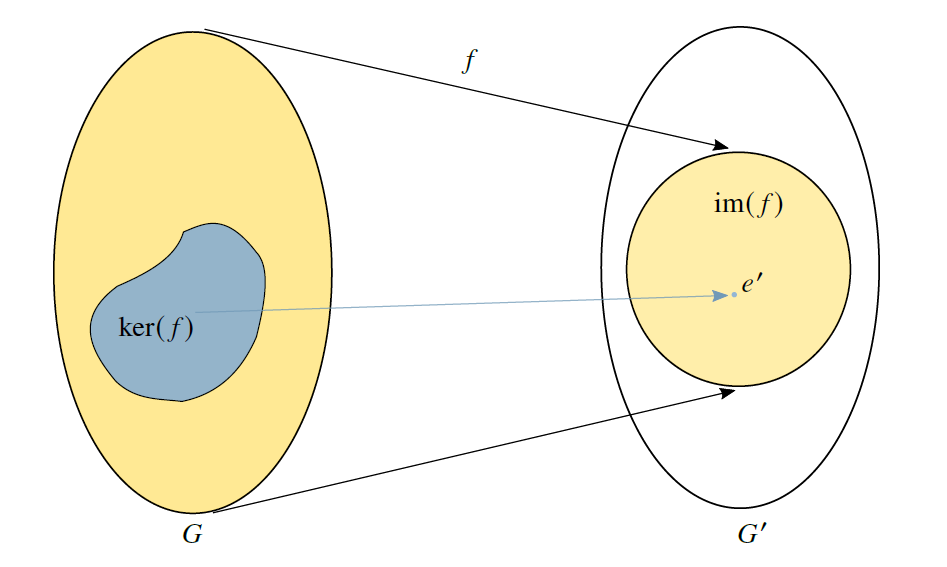
\includegraphics[scale=0.35]{群同态的核与像示意图.png}
\label{figure:群同态的核与像示意图}
\caption{群同态的核与像示意图}
\end{figure}



\begin{proposition}\label{proposition:群同态的核是定义域的子群,像是陪域的子群}
令 $f:(G,\cdot)\to (G',*)$ 是一个群同态,则核是定义域的子群,像是陪域的子群,即
\begin{align*}
\ker(f) < G,\quad
\mathrm{im}(f) < G'.
\end{align*}
\end{proposition}
\begin{remark}
根据\hyperref[theorem:群同构第一定理]{群同构第一定理}进一步可知,$\ker f \lhd G$.但是注意同态的像($\mathrm{im}(f)$)未必是$G'$的正规子群,往往只是普通的子群。
\end{remark}
\begin{proof}
先证明第一个子群关系。我们利用 $f(e)=e'$ 来说明 $e\in\ker(f)$。接着,设 $x,y\in\ker(f)$,只需证明 $xy^{-1}\in\ker(f)$。利用同态的性质,$f(xy^{-1}) = f(x)f(y)^{-1}=e'e'^{-1}=e'$,这就证明了 $xy^{-1}\in\ker(f)$。第一个子群关系得证。

再证明第二个子群关系。同样由于 $f(e)=e'$,我们有 $e'\in\mathrm{im}(f)$。接着,设 $y = f(x),y' = f(x')\in\mathrm{im}(f)$,只需证明 $yy'^{-1}\in\mathrm{im}(f)$。同样利用同态的性质,$yy'^{-1}=f(x)f(x')^{-1}=f(xx'^{-1})\in\mathrm{im}(f)$。第二个子群关系也得证。这样我们就证完了整个命题。
\end{proof}

\begin{example}
证明:$(SL(n,\mathbb{R}),\cdot)<(GL(n,\mathbb{R}),\cdot)$.
\end{example}
\begin{proof}
由\hyperref[proposition:行列是就是一个乘法群同态]{命题\ref{proposition:行列是就是一个乘法群同态}}可知,$\det : GL(n, \mathbb{R}) \to (\mathbb{R}^\times, \cdot)$ 是一个乘法群同态.注意到$\ker (det)=(SL(n,\mathbb{R}),\cdot)$,因此由\hyperref[proposition:群同态的核是定义域的子群,像是陪域的子群]{命题\ref{proposition:群同态的核是定义域的子群,像是陪域的子群}}可知,$(SL(n,\mathbb{R}),\cdot)=\ker (det)<(GL(n,\mathbb{R}),\cdot)$.
\end{proof}

\begin{definition}[满同态与单同态]
令 $f:(G,\cdot)\to (G',*)$ 是一个群同态,我们称 $f$ 是一个\textbf{满同态}当 $f$ 是满射,称 $f$ 是一个\textbf{单同态}当 $f$ 是单射。 
\end{definition}

\begin{proposition}\label{proposition:一个群同态是单的当且仅当核是平凡的}
令 $f:(G,\cdot)\to (G',*)$ 是一个群同态,则
\begin{enumerate}
\item $f$ 是一个单同态当且仅当 $\ker(f)=\{e\}$。也就是说,一个群同态是单的当且仅当核是平凡的。

\item $f$ 是一个满同态当且仅当 $ \mathrm{im}(f)=G'$。也就是说,一个群同态是满的当且仅当值域等于陪域。
\end{enumerate}
\end{proposition}
\begin{proof}
\begin{enumerate}
\item 假设 $f$ 是单的,那么因为 $f(e)=e'$,因此若 $f(x)=e'$,则利用单射的性质我们一定有 $x = e$,这就证明了核是平凡的。(这个方向是显然的)

另一个方向不那么显然。我们假设 $\ker(f)=\{e'\}$。假设 $x,x'\in G$,使得 $f(x)=f(x')$,我们只须证明 $x = x'$。在这里,我们同时右乘 $f(x')^{-1}$,得到 $f(x)f(x'^{-1})=f(xx'^{-1})=e'$。而因为核是平凡的,所以必须有 $xx'^{-1}=e$。接下来同时右乘 $x'$,我们就得到 $x = x'$。这就证明了这个命题.

\item 因为$f$是满同态,所以对$\forall a'\in G'$,都存在$a\in G$,使得$f(a)=a'.$故$a'\in \mathrm{im}(f)$.因此$G' \subset \mathrm{im}(f).$.又显然有$\mathrm{im}(f) \subset G'.$故$\mathrm{im}(f) = G'.$
\end{enumerate}
\end{proof}

\begin{figure}[H]
\centering
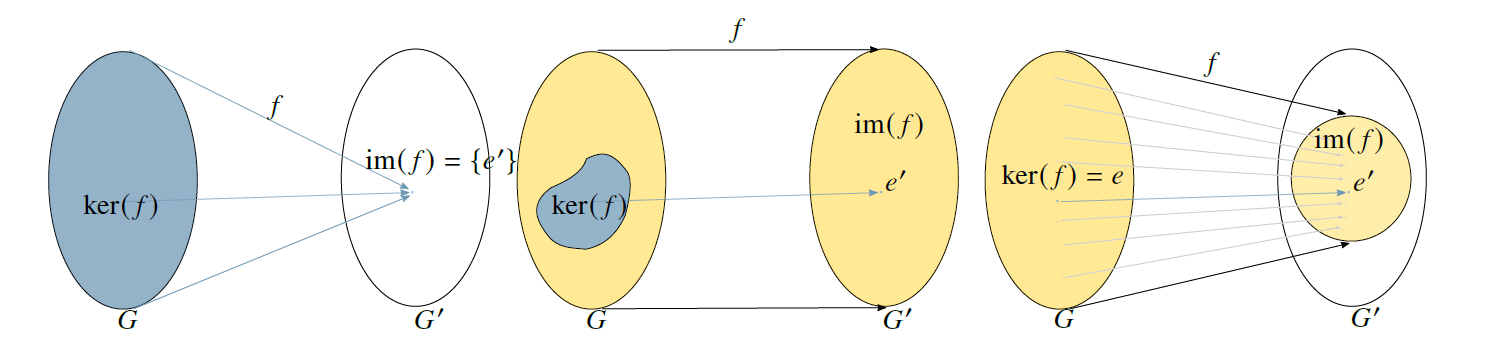
\includegraphics[scale=0.4]{平凡群,满同态和单同态示意图.png}
\label{figure:平凡群,满同态和单同态示意图}
\caption{平凡群,满同态和单同态示意图}
\end{figure}


\begin{example}\label{example:行列是就是一个乘法群同态}
证明:$\det : GL(n, \mathbb{R}) \to (\mathbb{R}^\times, \cdot)$ 是一个乘法群同态,并且是满同态,$\ker (\det)=SL(n, \mathbb{R}).$
\end{example}
\begin{proof}
设 \(A, B \in GL(n, \mathbb{R})\),则由行列式的 Laplace 定理可知 \(\det(AB) = \det(A)\det(B)\)。故 \(\det\) 是群同态。

任取 \(a \in \mathbb{R}^{\times}\),令 \(C = \begin{pmatrix}
a & & & \\
& 1 & & \\
& & \ddots & \\
& & & 1
\end{pmatrix}\),则 \(C \in GL(n, \mathbb{R})\) 并且 \(\det(C) = a\)。故 \(\det\) 是满同态。

一方面,任取 \(N \in SL(n, \mathbb{R})\),则 \(\det(N) = 1\),从而 \(N \in \mathrm{ker}(\det)\)。于是 \(SL(n, \mathbb{R}) \subset \mathrm{ker}(\det)\)。另一方面,任取 \(M \in \mathrm{ker}(\det)\),则 \(\det(M) = 1\),从而 \(M \in SL(n, \mathbb{R})\)。于是 \(\mathrm{ker}(\det) \subset SL(n, \mathbb{R})\)。故 \(\mathrm{ker}(\det) = SL(n, \mathbb{R})\)。 
\end{proof}

\begin{definition}[群同构]
令 $f:(G,\cdot)\to (G',*)$ 是一个映射,我们称 $f$ 是一个\textbf{群同构},当 $f$ 既是一个双射,又是一个群同态。简单来说,同构就是双射的同态。
\end{definition}

\begin{proposition}[群同构的逆也是群同构]\label{proposition:群同构的逆也是群同构}
若 $f:(G,\cdot)\to (G',*)$ 是一个群同构,则 $f^{-1}$ 也是群同构。
\end{proposition}
\begin{proof}
因为 $f^{-1}$ 也是双射,所以我们只须证明 $f^{-1}$ 是群同态。令 $x',y'\in G'$,设 $x' = f(x),y' = f(y)$。则 $x'*y' = f(x\cdot y)$,$x=f^{-1}(x'),y=f^{-1}(y')$,故 $f^{-1}(x'*y')=x\cdot y = f^{-1}(x')\cdot f^{-1}(y')$。这就完成了证明。 
\end{proof}

\begin{definition}[两个群的直积]
令 $(G,\cdot_1),(G',\cdot_2)$ 是两个群,我们记$(G\times G',*)$为$(G,\cdot_1)$和$(G',\cdot_2)$的\textbf{直积}.满足对于 $(x,y),(x',y')\in G\times G'$,有
\begin{align*}
(x,y)*(x',y')=(x\cdot_1 x',y\cdot_2 y').
\end{align*}
\end{definition}

\begin{proposition}[两个群的直积仍是群]\label{proposition:两个群的直积仍是群}
若 $(G,\cdot_1),(G',\cdot_2)$ 是两个群,则它们的直积 $(G\times G',*)$ 还是一个群。
\end{proposition}
\begin{proof}
封闭性:因为 $G$ 在 $\cdot_1$ 下封闭,$G'$ 在 $\cdot_2$ 下封闭,而 $G\times G'$ 的元素乘积是逐坐标定义的,则 $G\times G'$ 在 $* = (\cdot_1,\cdot_2)$ 下也是封闭的。

结合律:同样,逐坐标有结合律,故整体也有结合律。

单位元:设$e,e'$分别是$(G,\cdot_1),(G',\cdot_2)$的单位元,则不难想象,$(e,e')$ 是直积的单位元。对于任意 $(x,y)\in G\times G'$,我们有 $(x,y)*(e,e')=(x\cdot_1 e,y\cdot_2 e')=(x,y)$,另一边也是同理,这就证明了 $(e,e')$ 是直积的单位元。

逆元:对于任意 $(x,y)\in G\times G'$,设$x^{-1},y^{-1}$分别是$x,y$的逆元,则同样不难想象,$(x^{-1},y^{-1})$ 是 $(x,y)$ 的逆元。 
\end{proof}

\begin{definition}[一族群的直积]
令 $(G_i,\cdot_i)_{i\in I}$ 是一族群,其中 $I$ 是一个指标集。我们记它们的\textbf{直积}为 $(\prod_{i\in I}G_i,*)$.满足对于 $(x_i)_{i\in I},(y_i)_{i\in I}\in\prod_{i\in I}G_i$,有
\begin{align*}
(x_i)_{i\in I}*(y_i)_{i\in I}=(x_i\cdot_i y_i)_{i\in I}.
\end{align*}
\end{definition}

\begin{proposition}[一族群的直积仍是群]\label{proposition:一族群的直积仍是群}
若 $(G_i,\cdot_i)_{i\in I}$ 是一族群,则它们的直积 $(\prod_{i\in I}G_i,*)$ 还是一个群。  
\end{proposition}
\begin{note}
最经典的例子就是通过 $n$ 个实数加群 $(\mathbb{R},+)$ 直积得到的 $(\mathbb{R}^n,+)$.
\end{note}
\begin{proof}
证明与\hyperref[proposition:两个群的直积仍是群]{命题\ref{proposition:两个群的直积仍是群}}同理.封闭性与结合律是显然的。单位元是 $(e_i)_{i\in I}$,而 $(x_i)_{i\in I}$ 的逆元是 $(x_i^{-1})_{i\in I}$。 
\end{proof}

\begin{proposition}[一族Abel群的直积仍是Abel群]\label{proposition:一族Abel群的直积仍是Abel群}
若 $(G_i,\cdot_i)_{i\in I}$ 是一族Abel群,则它们的直积 $(\prod_{i\in I}G_i,*)$ 还是一个Abel群。  
\end{proposition}
\begin{proof}
由\hyperref[proposition:一族群的直积仍是群]{命题\ref{proposition:一族群的直积仍是群}}可知$(\prod_{i\in I}G_i,*)$ 还是一个群.下面证明它还是Abel群.

由$(G_i,\cdot_i)_{i\in I}$ 是一族Abel群可得,
对$\forall (x_i)_{i\in I},(y_i)_{i\in I} \in \prod_{i\in I}G_i$,都有
\begin{align*}
\left( x_i \right) _{i\in I}\cdot \left( y_i \right) _{i\in I}=\left( x_i\cdot _iy_i \right) _{i\in I}=\left( y_i\cdot _ix_i \right) _{i\in I}=\left( y_i \right) _{i\in I}\cdot \left( x_i \right) _{i\in I}.
\end{align*}
故$(\prod_{i\in I}G_i,*)$ 还是一个Abel群.
\end{proof}

\begin{definition}[投影映射]
若 $(G_i,\cdot_i)_{i\in I}$ 是一族群,$j\in I$ 是任意指标,我们定义映射到指标 $j$ 的\textbf{投影映射}为
\begin{align*}
p_j:\prod_{i\in I}G_i&\to G_j.
\end{align*}
对于 $(x_i)_{i\in I}$,我们称$p_j((x_i)_{i\in I})=x_j$为$(x_i)_{i\in I}$的\textbf{投影}.
\end{definition}

\begin{proposition}[投影映射是群同态]\label{proposition:投影映射是群同态}
若 $(G_i,\cdot_i)_{i\in I}$ 是一族群,$j\in I$ 是任意指标,则投影映射 $p_j:\prod_{i\in I}G_i\to G_j$ 是个群同态。
\end{proposition}
\begin{proof}
令 $(x_i)_{i\in I},(y_i)_{i\in I}\in\prod_{i\in I}G_i$,则
\begin{gather*}
p_j((x_i)_{i\in I})=x_j,\quad p_j((y_i)_{i\in I})=y_j\\
p_j((x_i)_{i\in I}*(y_i)_{i\in I})=p_j((x_i\cdot_i y_i)_{i\in I})=x_j\cdot_j y_j = p_j((x_i)_{i\in I})\cdot_j p_j((y_i)_{i\in I}).
\end{gather*}
\end{proof}






\end{document}